\documentclass[preprint,11pt,a4paper,times,doubleblind]{elsarticle}
\usepackage{amsmath,amssymb,bm}
\usepackage{graphicx}
\usepackage{booktabs}
\usepackage{array}
\usepackage{tabularx}
\usepackage[font=small,labelfont=bf]{caption}
\usepackage{microtype}
\usepackage{needspace}
\usepackage[hidelinks]{hyperref}
\graphicspath{{figs/}}
\setlength{\parskip}{2pt}
\setlength{\emergencystretch}{2em}

\renewcommand{\topfraction}{0.9}
\renewcommand{\bottomfraction}{0.8}
\renewcommand{\textfraction}{0.07}
\renewcommand{\floatpagefraction}{0.75}
\setcounter{topnumber}{3}
\setcounter{bottomnumber}{2}
\setcounter{totalnumber}{5}
\journal{International Journal of Heat and Mass Transfer}

\begin{document}

\begin{frontmatter}

\title{Field accuracy is not heat accuracy: wall-flux-constrained surrogates
for non-Boussinesq convection}

\author[a]{}
\address[a]{}
\hypersetup{pdfauthor={Anonymous}}

\begin{abstract}
Paired Boussinesq and compressible simulations are expensive, and public data sets fix the
relative temperature contrast $\varepsilon=\Delta T/T_0$. Such surrogates are usually
selected by relative $L_2$ field error. We show that, for steady two-dimensional
buoyancy-driven enclosure convection, this metric can rank a model above doing nothing on wall
heat transfer. On 200 held-out classical-cavity samples, a prior with a $0.09\%$ median field
error misses the both-wall integral Nusselt number by $2.0\%$ ($1.4$--$2.9\%$ across seeds), and
$42\%$ of the samples have a field error below $1\%$ and a $Nu$ error above $2\%$. A
22-sample random-wall replication at $\varepsilon\approx1.2$ gives $0.47\%$ field error and
$4.04\%$ $Nu$ error, with $66\%$ of the samples in the same region. A wall-flux penalty
reduces the both-wall error to $0.01\%$ on the classical cavity and $0.58\%$ in the replication,
and the local flux error to $0.08\%$ and $1.14\%$; the median field error moves from $0.09\%$ to
$0.10\%$ and from $0.47\%$ to $0.49\%$. The correction is largely a
redistribution of wall flux: at $\varepsilon=1.2$ the hot-wall integral $Nu$ changes by
$0.67\%$ while the local flux changes by $4.25\%$ in $L_1$. The underlying
correction factorises as $D=\varepsilon P(X)+O(\varepsilon^2)$ across 627 paired solutions with
$\varepsilon=0.02$--$1.9$; the velocity channels follow $R=A\varepsilon^m$ over the full window
with $m=1.023\pm0.018$ and $0.995\pm0.019$. A quadratic refinement gives positive curvature
$\kappa=0.70$ and $0.83$ (point estimates), and the prefactor $A$ is a functional of the flow.
The law makes a public single-contrast data set usable at $\varepsilon=0.2$--$1.9$ within its
boundary-condition family: a plain model trained at $\varepsilon_0=1.2$ and rescaled by
$\varepsilon/\varepsilon_0$ performs within $0.2\%$ of the factorized target, so applying
$\varepsilon$ outside the learned correction, rather than the residual parameterisation, carries
the transfer. At
$\varepsilon=1.9$ the integral $Nu$ change is $-5.1\%$ at $Ra=10^4$ and about $-2\%$ at
$Ra=10^5$--$10^6$. Inference takes 6.3\,ms; replacing the compressible member saves
$2.9\times$ per pair and $13\times$ for a 20-flow $\times$ 5-contrast scan.
\end{abstract}

\begin{keyword}
natural convection \sep Boussinesq approximation \sep low-Mach compressible flow \sep
physics-informed surrogate \sep data reuse \sep wall heat flux
\end{keyword}

\end{frontmatter}

\section*{Nomenclature}
\vspace{-0.5em}
\begin{center}\small
\setlength{\tabcolsep}{4pt}
\resizebox{\textwidth}{!}{%
\begin{tabular}{@{}p{1.1cm}p{6.1cm}p{1.1cm}p{6.1cm}@{}}
\toprule
\multicolumn{2}{@{}l}{\emph{Roman}} & \multicolumn{2}{l}{\emph{Greek}}\\
\midrule
$A$ & prefactor of $R=A\varepsilon^{m}$ & $\Delta T$ & wall-to-wall temperature contrast\\
$D$ & correction $Y-X$ & $\varepsilon$ & relative contrast, $\Delta T/T_0$\\
$Fr$ & Froude number, $Fr^{2}=\Delta T/T_0$ & $\theta$ & normalised temperature\\
$m$ & scaling exponent & $\kappa$ & curvature in $R=A\varepsilon(1+\kappa\varepsilon)$\\
$Ma$ & Mach number & $\rho$ & density\\
$Nu$ & Nusselt number & $\chi$ & base-flow advection strength\\
$p$ & pressure & & \\
$P,\,Q$ & first- and second-order correction fields & & \\
$Pr$ & Prandtl number & & \\
$R$ & relative correction, $\|Y-X\|/\|Y\|$ & & \\
$Ra$ & Rayleigh number & & \\
$Re$ & Reynolds number, $(Ra/Pr)^{1/2}$ & & \\
$T$ & temperature, $T_0$ its reference value & & \\
$\bm u$ & velocity, $(u_x,u_y)$ & & \\
$\hat u$ & peak Boussinesq speed & & \\
$X,\,Y$ & Boussinesq and compressible solutions & $\mathcal{L}$ & linearised low-Mach operator at $O(\varepsilon)$\\
\bottomrule
\end{tabular}}
\end{center}

\section{Introduction}
\label{sec:intro}

Steady natural convection is a workhorse of thermal engineering and it is expensive. A
converged pair of two-dimensional Boussinesq and compressible solves on a $64^2$ mesh costs
34\,s of wall clock on an eight-way desktop (Sec.~\ref{sec:cost}); three-dimensional problems
cost hours to days. Here the scaling law and the speed-up are measured in two dimensions; the
three-dimensional pairs are used only to check the exponent. Surrogate modelling removes this cost by learning the map from a cheap
model to an expensive one \citep{giacomini2026surrogates,meng2025physics}. For convection the
two models are not arbitrary fidelities: they are the Oberbeck--Boussinesq equations and the
low-Mach compressible equations. Boussinesq is exact only as the relative temperature contrast
vanishes; the difference is $O(\beta\Delta T)$ and has been characterised asymptotically for
decades \citep{spiegel1960boussinesq,gray1976validity}.

The numerical literature offers several ways to reduce the cost. Reduced-order models replace
the discretised equations by a small number of modes \citep{huhn2022parametric}; graph
convolutional networks exploit the mesh \citep{feng2024graph,peng2023physics}; operator
learning removes the mesh-resolution constraint
\citep{lu2021learning,wang2021learning,li2021fourier}, with applications to sparse-field
reconstruction \citep{zhao2023recfno} and heat-pipe startup \citep{yu2026fourier}.
Physics-informed neural networks take the opposite route and solve one instance by minimising a
residual \citep{raissi2019physics,cai2021physics,jalili2023physics,sahin2023deep}; reviews of
the numerical analysis and the application landscape are given by De Ryck and Mishra
\citep{deryck2024numerical} and Luo et al. \citep{luo2025physics}. These methods reduce the cost of a single query, but they still need
paired data at the operating conditions of interest.

Non-Oberbeck--Boussinesq effects have been measured under strong temperature contrast
\citep{yik2020turbulent}, in cryogenic helium \citep{macek2023assessing}, and in water-filled
cavities \citep{pan2023non}; at large contrast they can grow cold-corner vortices and reverse
the large-scale circulation \citep{xia2016flow}. The heat-transfer and large-scale dynamics of
Rayleigh--B\'enard convection are reviewed by Ahlers et al. \citep{ahlers2009heat}. Low-Mach formulations for enclosed thermal
convection have been developed and compared with the Boussinesq limit
\citep{zhang2023investigation,satake2024mathematical}, and the rigorous derivation of the
Oberbeck--Boussinesq system has been revisited \citep{bella2023rigorous}. These studies fix the
contrast and compare the two solutions. They do not extract its dependence as a reusable scaling.

The practical difficulty appears when a surrogate is trained on a paired data set at a single
contrast. Menglik et al. \citep{menglik2026neural} released 4000 paired
Boussinesq$\to$compressible steady
solutions in two dimensions, with three held-out splits, at one value of
$\varepsilon=\Delta T/T_0=1.2$. A network trained on that release learns the correction at
$\varepsilon=1.2$. At another contrast the Boussinesq input is unchanged, because the
Boussinesq equations do not contain $\varepsilon$, while the correction that must be added
scales with $\varepsilon$. The network has no signal with which to rescale what it memorised.
The usual remedy is a second paired data set, which pays again the cost the surrogate was meant
to remove.

This paper removes that barrier. The correction between the two members factorises. An
$\varepsilon$-expansion of the compressible member gives the Boussinesq system at $O(1)$ and a
linear, $\varepsilon$-independent operator at $O(\varepsilon)$. Hence
\begin{equation}
  D=Y-X=\varepsilon P(X)+\varepsilon^2 Q(X)+\cdots,
  \label{eq:factor}
\end{equation}
so a surrogate only has to learn the spatial shape $P$, and $\varepsilon$ can be applied
outside the network. The same expansion identifies the parameter that controls the gap:
$Fr^2=\varepsilon$ identically in the non-dimensionalisation used by the released data and by
our solver, while $Ma$ enters the retained equations only at $O(Ma^2)$. The break-symmetry
axis is therefore one-dimensional.

We test the consequence on 627 paired solutions in the unit square, on a second geometry, on a
second Prandtl number, on 33 three-dimensional pairs, and on two public data sets generated
independently of our solver. The law holds for the velocity and pressure channels; the temperature channel has a
flow-dependent amplitude that collapses on the peak Boussinesq speed. The scaling law makes a
single-contrast public data set reusable within its boundary-condition family, and the limit
is equally clear: the law transfers the $\varepsilon$ dependence, not the flow-dependent
prefactor.

The central result, however, is not the law by itself. The correction is largely a
redistribution of wall flux: at $\varepsilon=1.2$ the integral Nusselt number of the classical
cavity changes by $0.67\%$ on the hot wall while the local wall flux changes by $4.25\%$ in $L_1$. A surrogate
can therefore reproduce the temperature field to $0.47\%$ in relative $L_2$ and still miss the
integral $Nu$ by $4\%$. On the 22 held-out random-wall samples at $\varepsilon=1.1$--$1.3$,
$66\%$ of the field-only predictions have a field error below $1\%$ and a $Nu$ error above
$2\%$; on the 200 cavity samples, $42\%$ do. Relative $L_2$ is
not a sufficient selection metric for a heat-transfer surrogate. A wall-flux penalty in the
training loss reduces the heat-transfer bias at a small cost in field error.

The contributions are:
\begin{enumerate}
\item a per-sample demonstration that relative $L_2$ field accuracy does not imply
Nusselt-number accuracy, with a mechanism: the correction redistributes the wall-normal
temperature gradient while the integral almost cancels;
\item a wall-flux training penalty that reduces the both-wall $Nu$ error from $4.0\%$ to
$0.58\%$ on the random-wall replication ($0.01\%$ on the classical cavity), and the local
wall-flux error to $1.2\%$ or below;
\item a quantitative law for the Boussinesq--compressible gap, $R=A\varepsilon^m$ with
$m$ indistinguishable from one over the full window and a positive quadratic curvature,
calibrated over two decades of $\varepsilon$ and tested across geometry, fluid and
dimensionality, together with a within-family data-reuse rule. The factorized target is one
implementation; applying the known $\varepsilon$ scaling is what makes the data reusable, so
the factorisation, not the network, is the reusable object.
\end{enumerate}

The main sweep is two-dimensional and steady. The three-dimensional check uses 33 pairs at three
Rayleigh numbers and one resolution; it tests the exponent, not a three-dimensional design
workflow. The scope is stated in Sec.~\ref{sec:discussion}.

\section{Physical scaling}
\label{sec:theory}

\subsection{Two members and one contrast parameter}

Each sample is a paired steady solution of one configuration. The high-fidelity member $Y$ is
the low-Mach compressible formulation in $(\bm u,T,\rho,p)$:
\begin{align}
  \nabla\cdot(\rho\bm u)&=0,\label{eq:mass}\\
  \nabla\cdot(\rho\bm u\otimes\bm u)&=-\nabla p+\frac{1}{Re}\nabla\cdot\bm\sigma
  -\frac{1}{Fr^2}\rho\bm g,\label{eq:mom}\\
  \nabla\cdot(\rho E\bm u)&=\frac{\gamma}{Re\,Pr}\nabla^2 e
  +\nabla\cdot(\bm P_{\mathrm{work}}\bm u)+O(Ma^2),\label{eq:energy}\\
  \rho e&=\gamma Ma^2p+1,\qquad Re=(Ra/Pr)^{1/2}.\label{eq:eos}
\end{align}
The low-fidelity member $X$ is the Boussinesq system in $(\bm u,T,p)$ on the same mesh:
\begin{align}
  \nabla\cdot\bm u&=0,\label{eq:bqmass}\\
  \bm u\cdot\nabla\bm u&=-\nabla p+\left(\frac{Pr}{Ra}\right)^{1/2}\nabla^2\bm u
  +\theta\bm g,\label{eq:bqmom}\\
  \bm u\cdot\nabla\theta&=(Ra\,Pr)^{-1/2}\nabla^2\theta,\qquad
  \theta=\frac{T-T_0}{\Delta T}.\label{eq:bqtemp}
\end{align}
Both members use Taylor--Hood-type mixed elements, damped Newton iterations and a MUMPS
factorisation. They start from the same initial field and the same wall-temperature seed, so
they follow the same branch. The wall data are random Fourier temperatures with per-wall mode
dials; the classical differentially heated cavity is the one-mode member of the same family.

The generator draws $Ra$ and $\varepsilon$ independently. At fixed $Ra$, changing
$\varepsilon$ changes $Fr=\sqrt{\varepsilon}$, the buoyancy scale, while $Re$, $Pr$ and
$\gamma$ stay fixed. The Boussinesq member sees only $Ra$ and the thermal boundary data. This
is a statement about the dimensionless parameterisation; a fixed apparatus follows the
one-dimensional slice $Ra\propto\varepsilon$, while the $(Ra,\varepsilon)$ rectangle contains
that slice.

Two simplifications follow from the equations. First, $Fr^2=\beta\Delta T=\Delta T/T_0$
identically in this non-dimensionalisation, so $Fr$ is not a second free axis. Second, $Ma$
appears only at $O(Ma^2)$ in the retained low-Mach system. A 24-fold change in $Ma$ at fixed
$Ra$, $T_0$ and $\Delta T$ leaves the measured correction unchanged to a relative $10^{-5}$,
which is the precision of the solve. The free parameter is $\varepsilon$.

The Boussinesq solution is $\varepsilon$-blind to solver precision. Neither $T_0$ nor $\Delta T$ appears
alone in Eqs.~\eqref{eq:bqmass}--\eqref{eq:bqtemp}; with the thermal data prescribed in
$\theta$ and $Ra$ fixed, $X$ cannot depend on $\varepsilon$. Across 20 configurations
$\times$ 5 contrasts, the maximum relative deviation of $X$ is $9.77\times10^{-8}$, the
solver's convergence floor. The amplitude of the correction is thus set by a variable that is
absent from the input. The spatial shape remains a function of $X$ and is learnable.

\subsection{Why the correction factorises}

Write $T=T_0(1+\varepsilon\theta)$ with $\theta=O(1)$ and use $\rho=1/T$. The buoyancy source
becomes
\begin{equation}
  \frac{\rho\bm g}{Fr^2}=\frac{\rho\bm g}{\varepsilon}
  =\frac{\bm g}{\varepsilon}-\theta\bm g+\varepsilon\theta^2\bm g+\cdots.
  \label{eq:buoy}
\end{equation}
The constant $\bm g/\varepsilon$ is balanced by a hydrostatic pressure $p_{-1}/\varepsilon$
with $\nabla p_{-1}=-\bm g$, which drops out at the next order. The $O(1)$ balances are
\begin{align}
  \nabla\cdot\bm u_0&=0,\label{eq:o1mass}\\
  \bm u_0\cdot\nabla\bm u_0&=-\nabla\tilde p_0+Re^{-1}\nabla^2\bm u_0+\theta_0\bm g,\\
  \bm u_0\cdot\nabla\theta_0&=(Re\,Pr)^{-1}\nabla^2\theta_0,\label{eq:o1temp}
\end{align}
which is term-by-term the Boussinesq system solved as $X$, with
$Re^{-1}=(Pr/Ra)^{1/2}$. The correction at $O(\varepsilon)$ is driven by the density
modulation:
\begin{align}
  \nabla\cdot\bm u_1&=\nabla\cdot(\theta_0\bm u_0),\label{eq:div1}\\
  \nabla\cdot(\bm u_1\otimes\bm u_0+\bm u_0\otimes\bm u_1
  -\theta_0\bm u_0\otimes\bm u_0)
  &=-\nabla\tilde p_1+Re^{-1}\nabla^2\bm u_1+\theta_1\bm g-\theta_0^2\bm g.
  \label{eq:mom1}
\end{align}
The mass equation is inhomogeneous, so the operator is not the Boussinesq operator
linearised about $X$; it is the linearisation of the retained low-Mach system about $X$, with
the mass constraint carried inside. Its only singular mode is the constant pressure, and the
compatibility condition holds because $\bm u_0\cdot\bm n=0$ on the walls. Since the operator
is built from $X$ and contains no explicit $\varepsilon$,
\begin{equation}
  D=-\varepsilon\mathcal L^{-1}S_1[X]-\varepsilon^2\mathcal L^{-1}S_2[X]+\cdots
  =\varepsilon P(X)+\varepsilon^2 Q(X)+\cdots.
  \label{eq:expansion}
\end{equation}

Five predictions follow: $R\to0$ as $\varepsilon\to0$; $R\propto\varepsilon$ with a vanishing
intercept; the shape of $D$ does not rotate with $\varepsilon$;
$\nabla\cdot\bm u_1=\nabla\cdot(\theta_0\bm u_0)$; and the $\varepsilon^1$ term carries most
of the correction energy. All five hold numerically (Supplementary Material). The
$\varepsilon^1$ term carries 86\% of the correction energy, $\varepsilon^1+\varepsilon^2$
carries 99.0\%, and three terms carry 99.9\% over the sampled range. The divergence identity
has cosine $0.994$ for $\varepsilon<0.6$ and $0.901$ at $\varepsilon=1.9$; the drop is the
footprint of the $\varepsilon^2$ term.

The expansion is valid for $\varepsilon<2$, because the cold wall
$T_c=T_0-\Delta T/2$ must remain positive. At $\varepsilon=1.9$, $T_c/T_0=0.05$, so the
density expansion is close to its limit. This is the quantitative boundary of the law, not a
fitting choice.

\subsection{The measured law}
\label{sec:law}

The calibration set contains 600 random-boundary samples with
$Ra\sim\log U[10^2,10^6]$, $\varepsilon\sim U[0.2,1.9]$ and 134 wall-mode families, plus 27
low-contrast checks at $\varepsilon=0.02,0.05,0.10$ and $Ra=10^3,10^4,10^5$. The 627 points
enter the fit; the low-contrast points anchor the $\varepsilon\to0$ end. The relative
correction is $R=\|Y-X\|/\|Y\|$.

Table~\ref{tab:law} and Fig.~\ref{fig:law} give the result. For $u_x$ and $u_y$ the free
power law returns $m=1.023\pm0.018$ and $0.995\pm0.019$. The pressure channel gives
$m=1.009\pm0.015$ in the fixed gauge described below; it is a numerical observation, not a
gauge-invariant exponent. The intercepts are consistent with zero. A quadratic fit
$R=a\varepsilon+c\varepsilon^2+b$ gives $c>0$ in all four channels with point estimates
$\kappa_{\rm fit}=c/a=0.70/0.83/0.42/0.73$ for $u_x/u_y/\theta/p$ (no confidence intervals are
available). A compact description is therefore
$R=A\varepsilon(1+O(\varepsilon))$ rather than an exact power. Fitting only
$\varepsilon\ge0.8$ returns $m=1.23$--$1.32$, the window average of the same curvature.

\begin{table}[htbp]
\centering
\caption{Power-law fit $R=A\varepsilon^m$ over the full two-decade window (627 samples). The
intercept is fitted separately on $\varepsilon\le0.5$. The pressure row uses the fixed gauge
of Sec.~\ref{sec:pressure}; its exponent is not gauge-invariant. $\theta$ is not included:
its free power-law fit is not identifiable, and its amplitude is discussed separately.}
\label{tab:law}
\setlength{\tabcolsep}{5pt}
\begin{tabular}{@{}lcccc@{}}
\toprule
channel & $A$ & $m$ & $R^2$ & intercept ($\varepsilon\le0.5$)\\
\midrule
$u_x$ & 0.147 & $1.023\pm0.018$ & 0.84 & $+0.0003\pm0.0047$\\
$u_y$ & 0.193 & $0.995\pm0.019$ & 0.82 & $+0.0030\pm0.0062$\\
$p$ & 0.148 & $1.009\pm0.015$ & 0.87 & $+0.0016\pm0.0030$\\
\bottomrule
\end{tabular}
\end{table}

\begin{figure}[htbp]
\centering
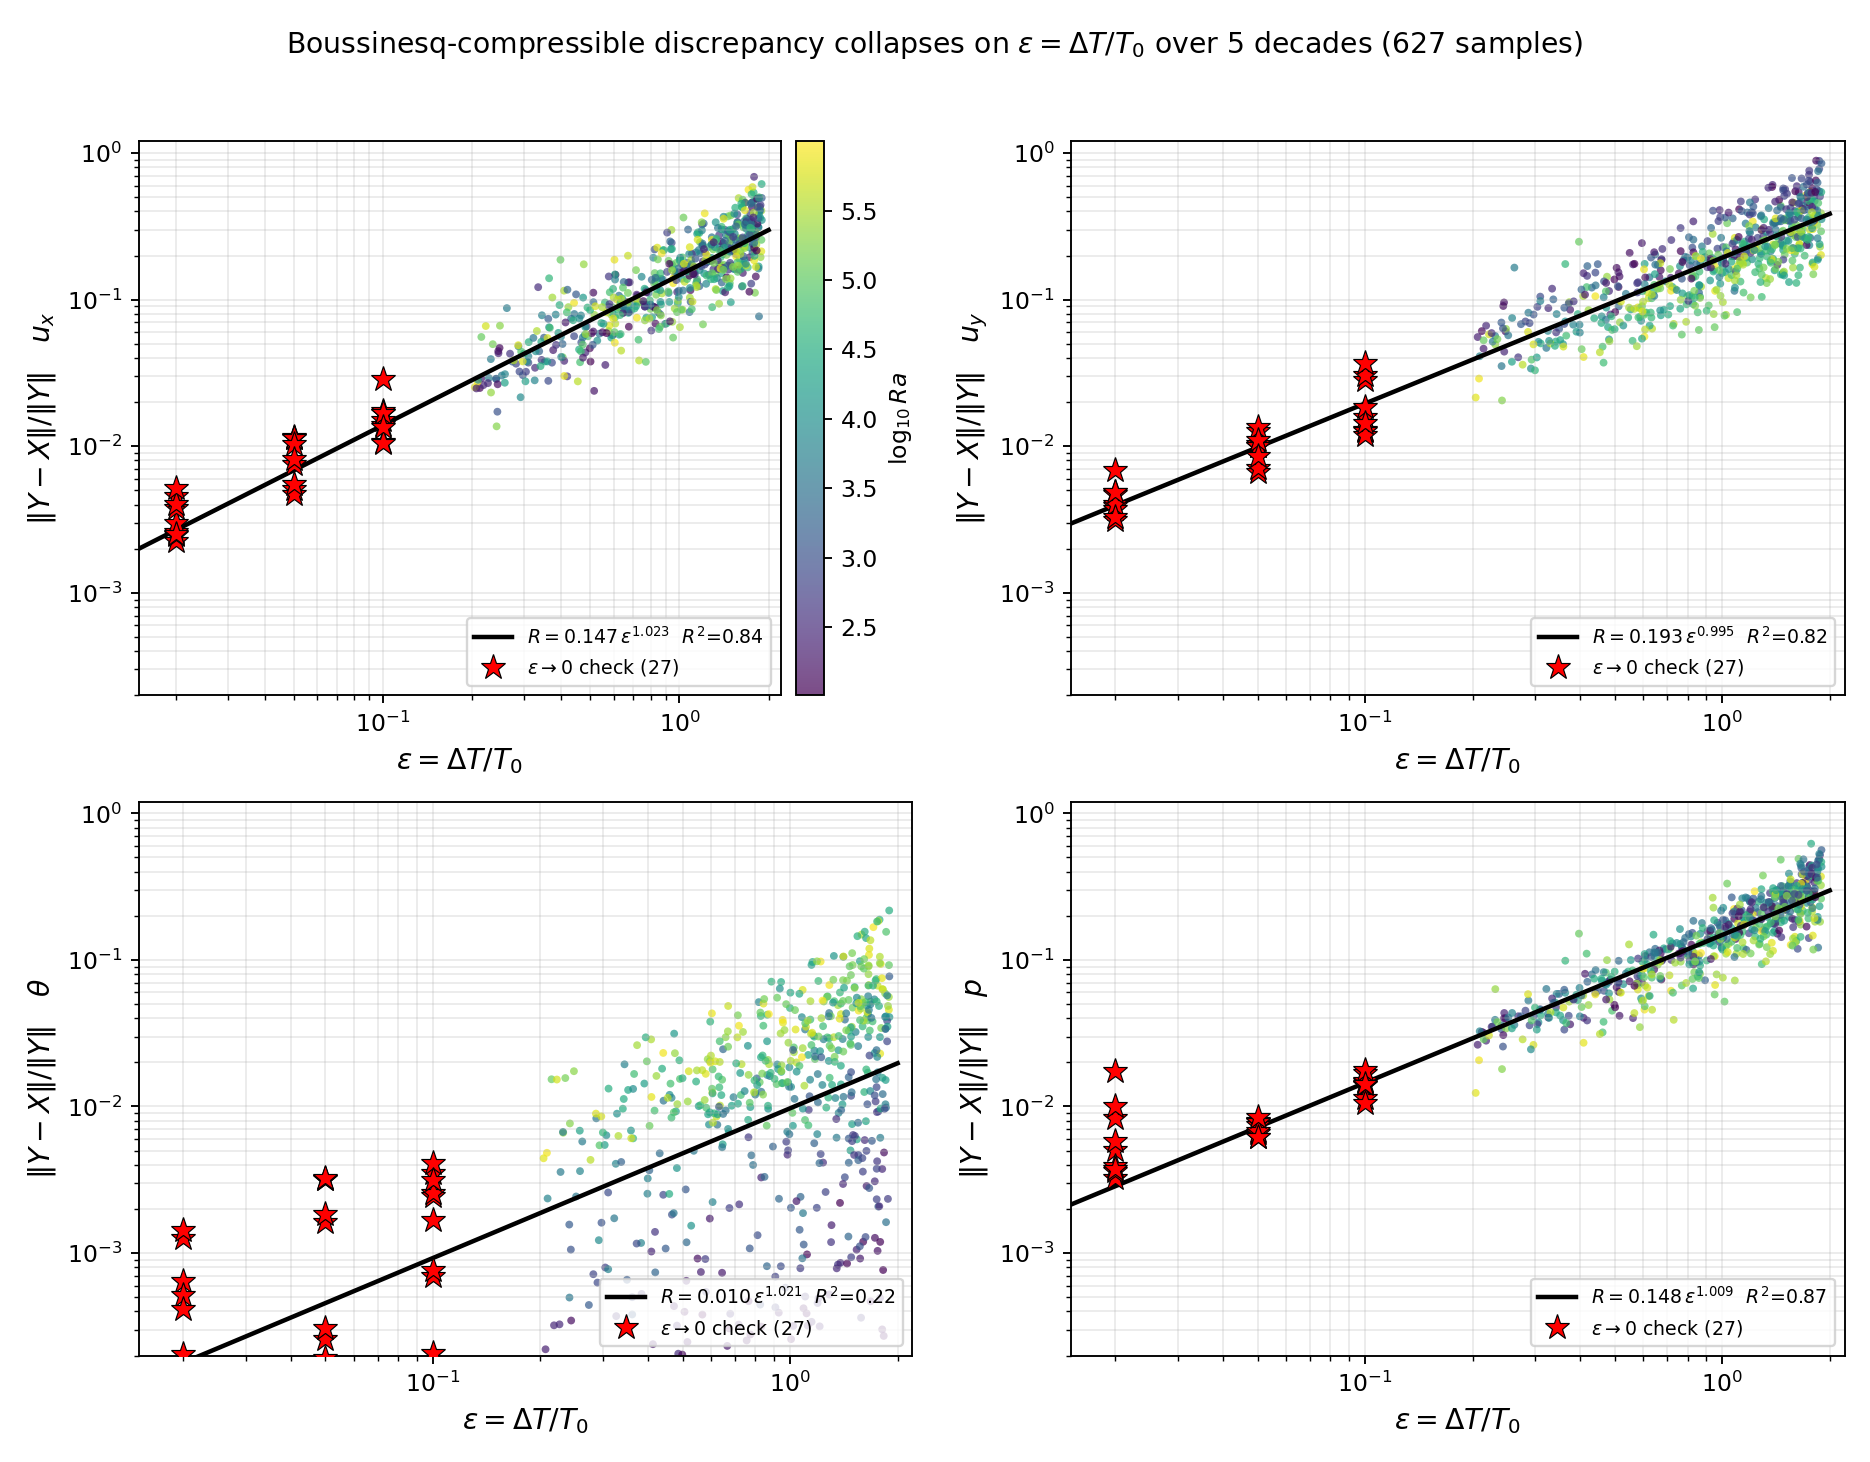
\includegraphics[width=0.82\textwidth]{fig1_law.png}
\caption{The Boussinesq--compressible discrepancy collapses on
$\varepsilon=\Delta T/T_0$ for $u_x$, $u_y$ and $p$ over two decades. The $\theta$ panel
scatters because its amplitude depends on the flow; it collapses on the peak Boussinesq speed
(Supplementary Material). Points: 600 random-boundary samples. Stars: 27 low-contrast checks.
Lines: power-law fits of Table~\ref{tab:law}.}
\label{fig:law}
\end{figure}

The temperature channel needs a flow-dependent amplitude. Its free power law has
$R^2=0.22$ and a slope that moves from 1.02 over the full window to 1.67 on the
104-configuration subset; the fitted amplitude is not predictive. This is not a failure of the
expansion. Writing $R_\theta/\varepsilon=c\hat u^a$, where $\hat u$ is the peak Boussinesq
speed available from $X$, collapses six data sets from two independent generators:
$a=1.86$--$1.98$ and $c=0.54$--$0.69$ for random-wall families,
$a=2.36$ and $c=2.06$--$2.10$ for the classical cavity. The classical cavity has a single
strong circulation with $\hat u$ 41\% above the random-wall median and 56\% above ours. The
same reading explains the residual scatter in $u_x$, $u_y$ and $p$: the prefactor is a
functional of the flow, and the flow is in the input $X$.

\subsection{What changes and what does not}
\label{sec:aspect}

The exponent is stable; the prefactor is not. In a 2:1 cavity with 104 samples, the
$\varepsilon$-only fit gives $m=1.09/1.16/0.93/1.08$ for $u_x/u_y/\theta/p$, within
0.3--1.8 combined standard errors of the unit-square values. The prefactor moves from
0.147/0.193/0.010/0.148 to 0.175/0.175/0.008/0.222. Changing the fluid from $Pr=0.71$ to
$Pr=4.38$ in 104 strictly paired configurations leaves the exponent within 1.5\% and the
\label{sec:water}
paired median $R$ within 5\%; the prefactor moves by at most 3.3\% except for pressure
(6.1\%). A 33-sample three-dimensional check at $Ra=10^4$, $3\times10^4$ and $10^5$ ($res=16$)
\label{sec:3d}
returns exponents for $u_x$, $u_y$ and $p$ of 1.09/1.05/1.14, 1.03/1.04/1.09 and 1.01/1.01/1.09, all within
0.15 of unity. The prefactor varies by factors of 2--13 across the three wall types.

The practical reading is simple. The law supplies the $\varepsilon$ dependence. It does not
supply the flow dependence. A surrogate must therefore take $X$ as input rather than a table
of $A$. This is also why transfer across boundary-condition families fails: the model has
learned one family's prefactor, not a universal constant.

\subsection{The pressure channel}
\label{sec:pressure}

The two members store pressure in different conventions. The compressible raw pressure
carries a hydrostatic ramp 12 times larger than its dynamic part, and the two weak forms use
opposite signs. Comparing raw pressures measures the conventions, not the flow. We subtract
the mean, remove a least-squares linear fit in the gravity direction, and flip the sign of the
Boussinesq member. Under this gauge the per-sample median of $|X_p|/|Y_p|$ is 0.960 and the
cosine is $+0.991$, against 0.929 and $+0.986$ for the public training set. The pressure
channel then follows the same law as the velocities, with $A=0.148$ and $m=1.009$. All
pressure numbers use this fixed gauge; the exponent is not gauge-invariant.

\section{Surrogate design}
\label{sec:method}

\subsection{Residual learning and the factorised target}
\label{sec:prior}

All surrogates use residual learning,
\begin{equation}
  \hat Y=X+N(X),
  \label{eq:residual}
\end{equation}
with a U-Net of width 32 or an FNO with 12 modes, width 32 and four layers (1.19M
parameters). Training uses Adam with cosine annealing, 200 epochs and batch 16. Inputs and
targets are scaled per channel by training-set standard deviations.

The prior changes the target, not the backbone. Instead of learning $D$, the network learns
$P=D/\varepsilon$ at the available contrast and the model returns
\begin{equation}
  \hat Y=X+\varepsilon N(X).
  \label{eq:prior}
\end{equation}
We compare five variants:
\begin{itemize}
\item A: $\varepsilon$-blind, target $D$;
\item B: $\varepsilon$ supplied as a constant input channel, target $D$;
\item P1: $\varepsilon$ supplied as input, target $D/\varepsilon$, multiplied outside;
\item P2: as P1 with a learned scalar curvature, $\varepsilon(1+\kappa\varepsilon)$;
\item P3: as P1 with no $\varepsilon$ input, so the network sees only $X$.
\end{itemize}
P1 is the most accurate form when $\varepsilon$ is known at training time. P3 is the form
that can be trained on a single-contrast data set and applied at another contrast; it must
infer the prefactor from the flow. The distinction is the difference between a model that
interpolates in $\varepsilon$ and one that reuses a data set.

\subsection{Wall-flux loss}

Field accuracy does not guarantee heat-transfer accuracy. For applications we add a relative
$L_1$ penalty on the wall-normal gradient,
\begin{equation}
  \mathcal L=\mathcal L_{\rm field}
  +\lambda\frac{\sum_{\rm wall}|\hat q-q|}{\sum_{\rm wall}|q|},
  \qquad q=-\frac{\partial\theta}{\partial n},
  \label{eq:fluxloss}
\end{equation}
with $\lambda=1$ and a six-point one-sided stencil. The same models are evaluated with two-,
four-, six- and eight-point stencils to separate the loss from the estimator.

\subsection{Data, splits and metrics}

The main data set is the 600-sample random-boundary scan, with the 27 low-contrast checks used
for the law. The paired scan contains 20 configurations $\times$ 5 contrasts; within a
configuration only $\varepsilon$ changes, so $X$ is identical and the error of any
$\varepsilon$-blind model is bounded exactly. The public release of Menglik et al.
\label{sec:public}
\citep{menglik2026neural}
provides 4000 random-wall pairs at $\varepsilon=1.2$, a 200-pair in-distribution test split,
a 200-pair out-of-distribution split with more complex wall dials, and 5000 + 200 classical
cavity pairs. The 2:1 cavity and the $Pr=4.38$ data are generated here with the same solver.

Two splits are used throughout: extrapolation (train $\varepsilon\le1.3$, test
$\varepsilon>1.3$, $n=218$) and interpolation (stratified 2:1 in $\varepsilon$, $n=200$).
Errors are per-channel relative $L_2$ against $Y$; the floor is $\hat Y=X$. Training uses
three seeds unless stated otherwise. When a model trained on one data set is applied to
another, the target is scaled by the source per-channel standard deviation; re-normalising by
the target's own standard deviation changes the temperature channel by $21\%$ and is not used.

\section{Results}
\label{sec:results}

\subsection{Field accuracy is not heat accuracy}
\label{sec:headline}

We first ask whether the metric used to select these surrogates is the right one.
Table~\ref{tab:headline} and Fig.~\ref{fig:fieldnu} compare, for the same 200 held-out
classical-cavity samples at $\varepsilon=1.2$, the per-sample relative $L_2$ error of the
temperature field with the per-sample error of the integral Nusselt number. The models are the
ones of Sec.~\ref{sec:transfer}: a U-Net trained on the 4000 public random-wall pairs at
$\varepsilon=1.2$ and applied without retraining to the classical-cavity split.

The field-only prior reduces the median field error from $8.4\%$ (returning $X$) to $0.09\%$.
Its median integral-$Nu$ error is $1.4$--$2.9\%$ across the three seeds,
against $0.48\%$ for returning $X$, and the fraction of samples with a field
error below $1\%$ and a $Nu$ error above $2\%$ ranges from $23\%$ to $82\%$. Within a seed the two errors are anti-correlated
(Spearman $-0.73$ for the seed shown in Fig.~\ref{fig:fieldnu}): the samples whose field looks
best are not the samples whose heat transfer is best. The wall-flux penalty moves the same
model back into the low-error region: median $Nu$ error $0.01\%$, local wall-flux error below
$0.1\%$, and field error $0.10\%$.

The pattern is not an artefact of crossing boundary-condition families. The full held-out
random-wall split has 200 samples, of which 22 lie at $\varepsilon=1.1$--$1.3$. On those 22, a
prior trained on the other 400 random-wall samples has a $0.47\%$ median temperature-field error
and a $4.04\%$ integral-$Nu$ error. The wall-flux penalty reduces the $Nu$ error to $0.58\%$ and
the local flux error from $4.94\%$ to $1.14\%$, while the field error moves from $0.47\%$ to
$0.49\%$. In $66\%$ of these samples the field error is below $1\%$ and the $Nu$ error above
$2\%$. The field norm is insensitive to the wall gradient in both families.

\begin{table}[htbp]
\centering
\caption{Field error versus wall heat transfer on 200 held-out classical-cavity samples at
$\varepsilon=1.2$. $T$ is the per-sample median relative $L_2$ error; the $Nu$
columns are the hot wall, cold wall, and both walls normalised by the true total; the last two
columns are the mean absolute wall-flux profile error and the fraction of
samples with $T<1\%$ and $Nu>2\%$. Values are means across three seeds; for the field-only
prior the both-wall error ranges from $1.4$ to $2.9\%$ and the fraction from $23$ to $82\%$.
The wall-flux row uses the penalty of Eq.~\eqref{eq:fluxloss}.}
\label{tab:headline}
\small
\setlength{\tabcolsep}{3.5pt}
\resizebox{\textwidth}{!}{%
\begin{tabular}{@{}lcccccc@{}}
\toprule
model & $T$ median & $Nu$ hot & $Nu$ cold & $Nu$ both & local flux & fraction\\
\midrule
return $X$ & 8.4\% & 0.67\% & 0.64\% & 0.48\% & 5.6\% & 0\%\\
field-only prior & 0.09\% & 2.0\% & 2.1\% & 2.0\% & 4.5\% & 42\%\\
prior + wall-flux & 0.10\% & \textbf{0.01\%} & \textbf{0.01\%} & \textbf{0.01\%} & \textbf{0.08\%} & 0\%\\
\bottomrule
\end{tabular}}
\end{table}

\begin{figure}[htbp]
\centering
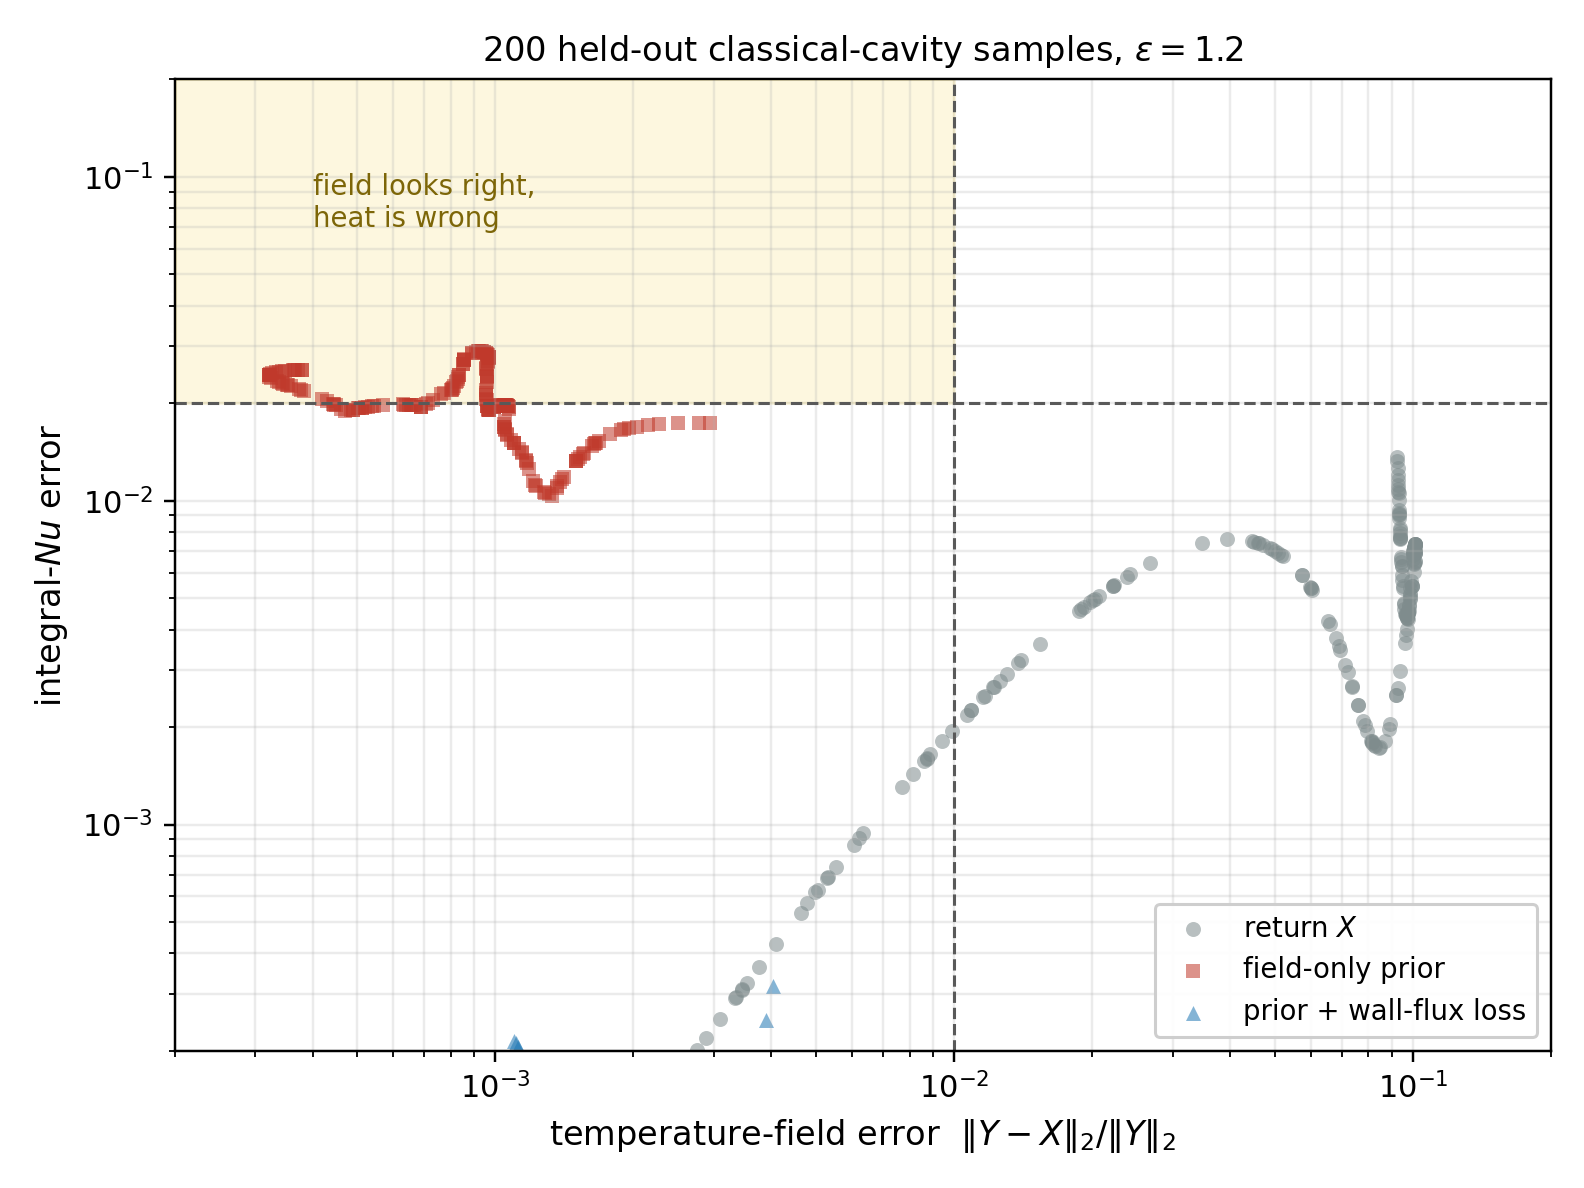
\includegraphics[width=0.78\textwidth]{fig_field_vs_nu.png}
\caption{Per-sample temperature-field error against integral-$Nu$ error for the 200 held-out
classical-cavity samples at $\varepsilon=1.2$. The shaded region is where a model looks accurate
in the field but is wrong in heat transfer. The field-only prior sits there; the wall-flux
penalty moves it out. Points are averages over three seeds; the prior's median $Nu$ error is
$1.4$--$2.9\%$ across seeds, and $42\%$ of the averaged samples lie in the shaded region.}
\label{fig:fieldnu}
\end{figure}

The mechanism is visible in the correction itself. The compressible member adds heat over the
lower half of the cavity and removes it over the upper half; the integral $Nu$ is the
$Nu$-weighted mean of this redistribution and almost cancels, while the wall-normal gradient
changes by several per cent. A field norm dominated by the interior does not see this
boundary-layer bias. Section~\ref{sec:nu} gives the per-wall breakdown, the stencil dependence
and the Rayleigh dependence.

\subsection{A single-contrast data set becomes reusable}
\label{sec:transfer}
\label{sec:reuse}

Table~\ref{tab:transfer} and Fig.~\ref{fig:transfer} show the central result. A plain U-Net
trained on the public 4000 random-wall pairs at $\varepsilon=1.2$ reaches $0.142$ in $u_x$ on
our extrapolation split, barely better than returning $X$ (0.3018). Applying the known
scaling to its output, $\hat Y=X+(\varepsilon/\varepsilon_0)N_{\rm plain}(X)$, reaches
$0.091$. Training the same architecture on $D/\varepsilon$ reaches $0.091$, within a few per
cent. The 1.55-fold gain over the unscaled plain model therefore comes from applying $\varepsilon$,
not from the network parameterization. The prior's value is that it makes the scaling explicit
and can be trained without $\varepsilon$ as an input.

Channel-averaged, the error falls from 0.131 to 0.085, a factor 1.5. Relative to returning
$X$, the channel average is $3.1\times$ lower ($3.3\times$ in $u_x$). The public prior is
better than the same prior trained on our own 382 samples (0.1250), because it sees ten times
more configurations.

\begin{table}[htbp]
\centering
\caption{Transfer from a single-contrast public data set to our
$\varepsilon\in[0.2,1.9]$ samples. Entries are relative $L_2$ errors for
$u_x/u_y/\theta/p$. Both public sets are at $\varepsilon\equiv1.2$. The ``own data'' row uses
382 training samples for extrapolation and 400 for interpolation, with the P3 prior (150
epochs, one seed). The ``plain, rescaled'' row applies
$\hat Y=X+(\varepsilon/\varepsilon_0)N_{\rm plain}(X)$ to the plain model's output; it is the
fair baseline for the prior. The public 4000 rows use three seeds; the 5000 rows use one, so
differences below 0.003 there are not resolved.}
\label{tab:transfer}
\small
\setlength{\tabcolsep}{4pt}
\begin{tabular}{@{}llccccc@{}}
\toprule
training data & model & split & $u_x$ & $u_y$ & $\theta$ & $p$\\
\midrule
do nothing & $\hat Y=X$ & extrap. & 0.3018 & 0.3731 & 0.0556 & 0.3320\\
 &  & interp. & 0.2203 & 0.2683 & 0.0381 & 0.2386\\
public 4000, random walls & plain & extrap. & 0.1417 & 0.1717 & 0.0225 & 0.1811\\
 &  & interp. & 0.1195 & 0.1437 & 0.0189 & 0.1422\\
public 4000, random walls & plain, rescaled & extrap. & 0.0912 & 0.1081 & 0.0118 & 0.1287\\
 &  & interp. & 0.0649 & 0.0766 & 0.0078 & 0.0871\\
public 4000, random walls & prior & extrap. & 0.0914 & 0.1080 & 0.0118 & 0.1287\\
 &  & interp. & 0.0651 & 0.0767 & 0.0077 & 0.0872\\
own data, random walls & prior & extrap. & 0.1250 & 0.1321 & 0.0170 & 0.1719\\
 &  & interp. & 0.0791 & 0.0811 & 0.0103 & 0.0947\\
public 5000, classical cavity & plain & extrap. & 0.3250 & 0.4007 & 0.0542 & 0.3167\\
 &  & interp. & 0.2937 & 0.3961 & 0.0555 & 0.3251\\
public 5000, classical cavity & prior & extrap. & 0.4078 & 0.4898 & 0.0715 & 0.3222\\
 &  & interp. & 0.3071 & 0.3643 & 0.0532 & 0.2487\\
\bottomrule
\end{tabular}
\end{table}

\begin{figure}[htbp]
\centering
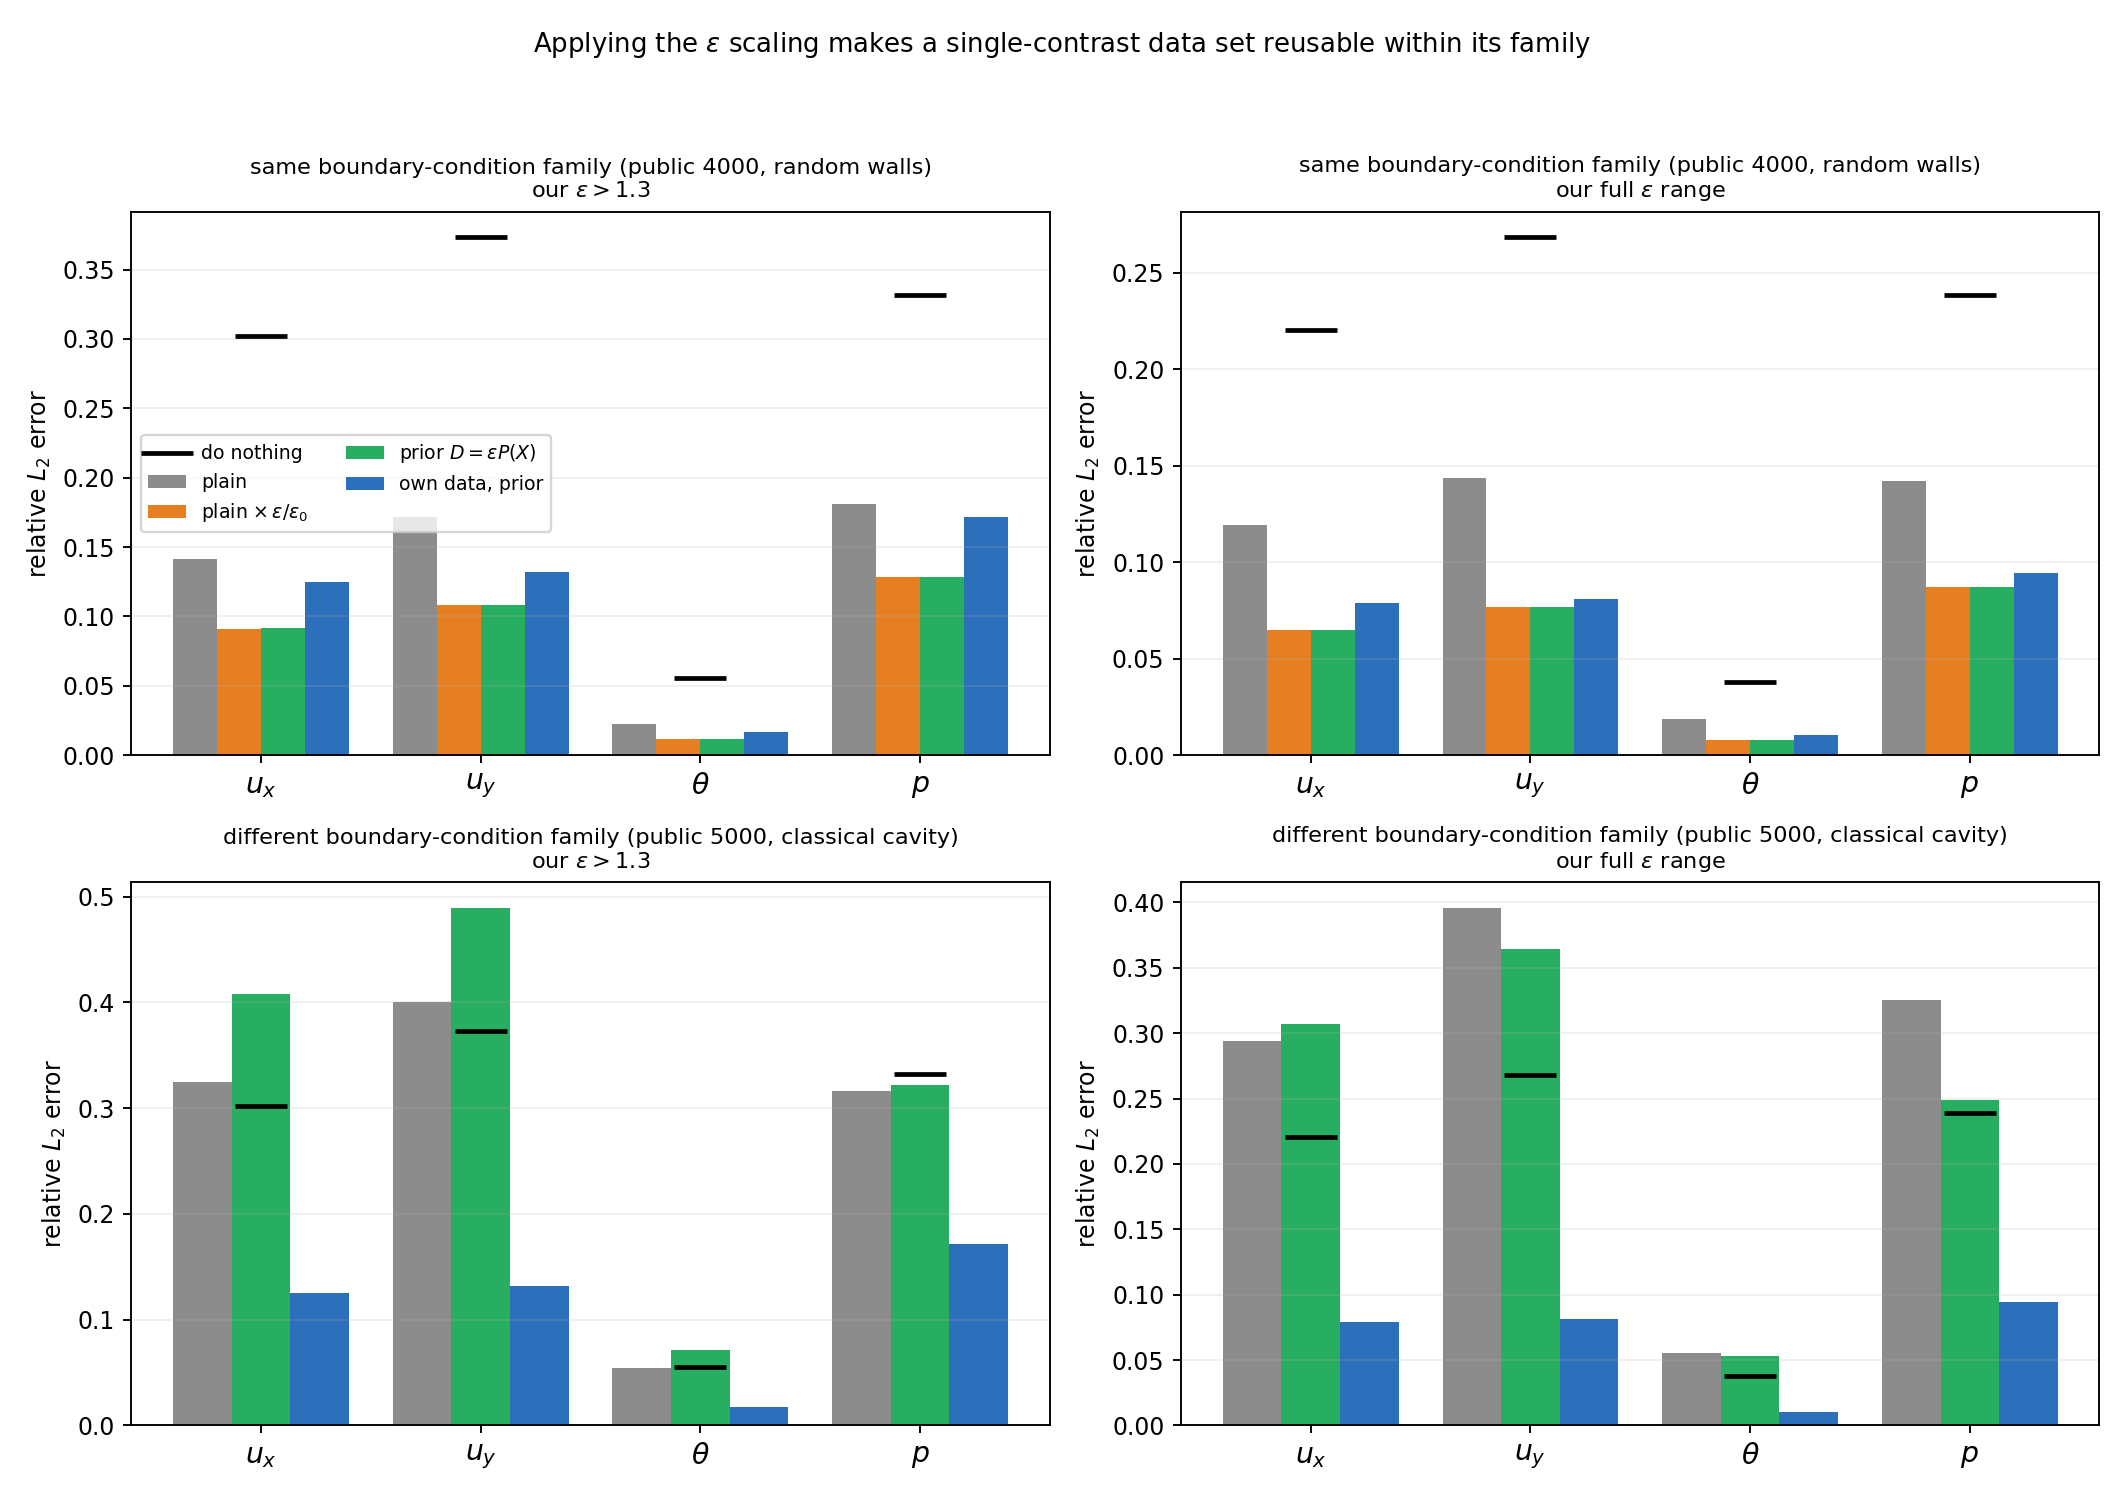
\includegraphics[width=0.95\textwidth]{fig6_transfer.png}
\caption{Reusing a single-$\varepsilon$ data set. Within the boundary-condition family the
prior transfers and beats the unscaled plain model; a plain model with the same scaling
applied outside performs within 0.2\% (Table~\ref{tab:transfer}). Across families the prior
fails and can be worse than returning $X$. The failure is the flow dependence of $A$, not the
$\varepsilon$ scaling. Public-data models are applied with the source per-channel
normalisation.}
\label{fig:transfer}
\end{figure}

Applying the scaling also changes the failure mode. The plain model's error at an unseen contrast grows
\label{sec:floor}
with the distance from the training contrast, because its correction is a fixed field. The
rescaled model's error stays proportional to the error in $P$, roughly uniformly in $\varepsilon$.

The paired scan makes the information limit explicit. Within one configuration $X$ is identical
for all five contrasts, so an $\varepsilon$-blind model must emit one field for all five. At
$\varepsilon=1.9$ the error is 0.388/0.575/0.060/0.424 for $\hat Y=X$,
0.243/0.295/0.031/0.273 for a model trained only at $\varepsilon=1.2$, and
0.209/0.268/0.028/0.235 for the unweighted $\varepsilon$-mean field
($u_x/u_y/\theta/p$, median over 20 configurations). No function of $X$ alone can beat the best
single field. The missing input is the scalar $\varepsilon$, not network capacity.

Across boundary-condition families the picture is different. Trained on the 5000 classical
cavity pairs, the plain model lands at 0.3250 in $u_x$, worse than the floor of 0.3018, so it
learns little that transfers. The prior is worse in extrapolation
(0.4078/0.4898/0.0715/0.3222) and does not beat returning $X$ in interpolation for
$u_x$, $u_y$ or $\theta$ (0.3071/0.3643/0.0532/0.2487). This is the predicted boundary: the prior carries the
$\varepsilon$ dependence, not another family's prefactor. The classical cavity's peak
Boussinesq speed is 41\% above the random-wall median, so $\hat u$ separates the families; it
does not order the per-sample error within a family (Spearman $-0.20$). It is a family-level
diagnostic, not a within-family transfer law.

The reverse direction is favorable for the field. The 4000 random-wall set contains the
one-mode classical cavity as a special case, and both plain and prior models trained on the
broad family reach 0.09--0.10\% relative $L_2$ on the 200 classical-cavity samples at
$\varepsilon=1.2$ (Table~\ref{tab:headline}), although their integral $Nu$ errors remain
1.4--2.9\% across seeds (2.0\% seed mean). The asymmetry is coverage, not a violation of the law: a model trained on a narrow
family cannot cover a broader one, while a model trained on a broad family can cover a
subfamily. This is the practical rule for choosing the training set.

The accuracy trade-off is visible when $\varepsilon$ is available at training time. On our own
\label{sec:blind}
data, P1 reaches $0.0937$ in $u_x$ in extrapolation, while P3 reaches $0.1214$; removing
$\varepsilon$ from the input costs accuracy but buys the ability to apply the model at another
contrast. The gap is the price of reuse. At small sample sizes the structured model is also
\label{sec:learning}
the cheaper one: at $n=50$ the prior is $1.4\times$ better than the $\varepsilon$-input network
in $u_x$ (0.1308 against 0.1831), and it remains ahead at $n=200$; the crossover is near
$n\approx300$ for $u_x$ and $u_y$, and $\theta$ never crosses. The prior at $n=200$ reaches
what the $\varepsilon$-input network needs about 270--290 samples to reach.

\subsection{Wall heat transfer: per-wall breakdown and Rayleigh dependence}
\label{sec:nu}
\label{sec:wall}

Table~\ref{tab:headline} splits the integral error by wall and adds the local profile error. The
hot-wall integral change between the two members is $0.67\%$ (cold wall $0.64\%$, both walls
$0.48\%$; mean per-sample hot-wall ratio $0.54\%$, median $0.58\%$), while the local wall flux is redistributed by $4.25\%$ in $L_1$ (p90 $7.33\%$,
pointwise excursions $\pm10\%$). The $4.25\%$ is the $L_1$ norm of the relative local change
$\Delta Nu(y)/Nu(y)$ between $X$ and $Y$. The $5.6\%$ entry in Table~\ref{tab:headline}
($6.0/5.2\%$ on the two walls) is the mean absolute error of the predicted wall-flux profile divided by its mean absolute value;
the two use different denominators and are not directly comparable.
The both-wall $2.0\%$ error is the flux-weighted combination of the per-wall $2.0\%$ (hot)
and $2.1\%$ (cold) values.

\begin{figure}[htbp]
\centering
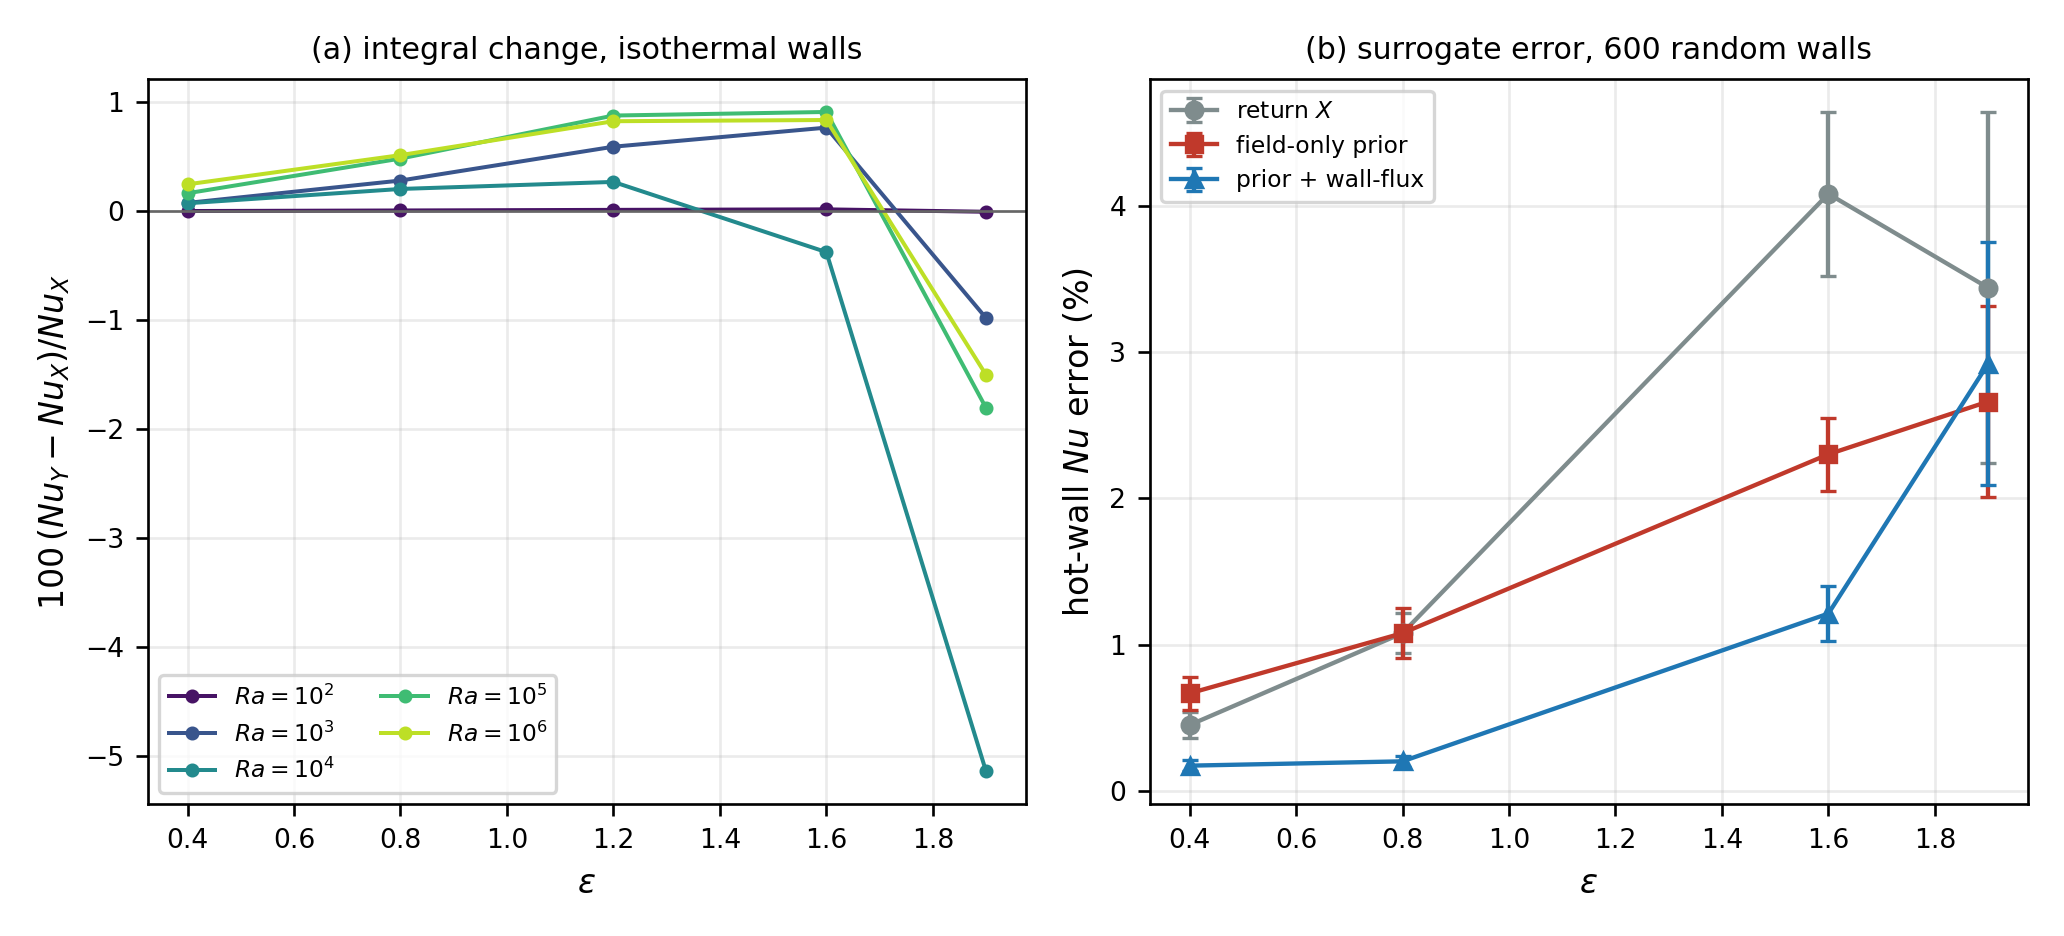
\includegraphics[width=0.95\textwidth]{fig_nu_eps_ra.png}
\caption{(a) Integral-$Nu$ change between the two members for the five isothermal-wall
configurations at $Ra=10^2$--$10^6$. The change is not a single function of $\varepsilon$: it
peaks at $-5.1\%$ at $Ra=10^4$ and is about $-2\%$ at higher $Ra$. (b) Hot-wall $Nu$ error of
the surrogate on the 600 random-wall samples. The wall-flux penalty reduces the error at
intermediate contrast; at $\varepsilon=1.9$ the improvement is not resolved.}
\label{fig:nu_eps_ra}
\end{figure}

The public prior reduces the median global temperature-field error from 8.4\% to 0.09\%, but
its hot-wall $Nu$ error is 2.0\% (1.4--2.9\% across seeds), larger than the 0.67\% of returning
$X$. The wall-normal derivative carries a bias that the field norm does not see. Adding the
wall-flux penalty brings the six-point integral error to 0.01\% and the local flux error to
0.08\%, at a cost of 0.01 percentage point in the median field error (0.09\% to 0.10\%).
With four- and eight-point stencils the same models give 0.3--0.9\%, against 1.8--3.6\% for the
field-only prior and 0.4--0.9\% for returning $X$; the ordering is stable, the absolute value
depends on the stencil. At $\varepsilon=0.4/0.8/1.6$ the penalty gives
0.17/0.20/1.21\% against 0.45/1.08/4.08\% for returning $X$; at $\varepsilon=1.9$ the gain is
not resolved.

The Rayleigh dependence is equally important. On the five isothermal-sidewall
configurations, the integral change at $\varepsilon=1.2$ spans $+0.01$ to $+0.87\%$. At
$\varepsilon=1.9$ the same five configurations give $-0.01$, $-0.98$, $-5.14$, $-1.81$ and
$-1.50\%$ for $Ra=10^2$, $10^3$, $10^4$, $10^5$ and $10^6$: the change peaks at $Ra=10^4$ and
is about $-2\%$ at higher $Ra$. A model calibrated on $Nu$ alone does not transfer across
$Ra$; the local field carries the correction. At $Ra=10^6$ the $256^2$ Boussinesq solution
gives $Nu=8.793$ on the hot wall, $0.37\%$ below the benchmark $8.825$ of Le Qu\'er\'e
\citep{lequere1991}; the $64^2$ and $128^2$ values are $8.563$ and $8.759$, so the grid
sequence approaches the benchmark.

\subsection{Cost}
\label{sec:cost}

Table~\ref{tab:cost} gives the wall-clock cost. A paired solve splits into a Boussinesq member
(median 11.7\,s) and a compressible member (22.3\,s). The surrogate replaces only the second.
Per pair the cost falls from 33.9\,s to 11.7\,s, a factor 2.9. For a single flow swept over
100 contrasts, one Boussinesq solve plus 100 inferences costs 16.6\,s against $3.77\times10^3$
for 100 compressible solves, a factor $2.3\times10^2$. For the 20-flow $\times$ 5-contrast
scan, the same-reuse comparison gives a factor 13. Inference takes 6.3\,ms on a GPU and
14.0\,ms on one CPU thread.

\begin{table}[htbp]
\centering
\caption{Wall-clock cost on the $64^2$ mesh. Solver rows use eight CPU threads; the surrogate
runs on an RTX 4060 Laptop GPU (batch 1) or one CPU thread. The 100-sample scan rows use that
scan's own timings; medians are not additive.}
\label{tab:cost}
\setlength{\tabcolsep}{4pt}
\begin{tabular}{@{}lcccc@{}}
\toprule
quantity & median & mean & p90 & max\\
\midrule
paired solve, 600 samples & 33.9\,s & 38.0\,s & 59.9\,s & 510\,s\\
Boussinesq member alone & 11.7\,s & 13.1\,s & 21.7\,s & ---\\
compressible member alone & 22.3\,s & 25.0\,s & 37.3\,s & ---\\
paired solve, 100-sample $\varepsilon$ scan & 55.8\,s & 67.7\,s & 136\,s & 202\,s\\
surrogate, GPU, batch 1 & 6.3\,ms & --- & --- & ---\\
surrogate, GPU, batch 256 & 0.49\,ms/sample & --- & --- & ---\\
surrogate, CPU, 1 thread & 14.0\,ms & --- & --- & ---\\
end-to-end pair (Boussinesq + surrogate) & 11.7\,s & --- & --- & ---\\
\bottomrule
\end{tabular}
\end{table}

\subsection{Why the scaling is not a fitting artefact}
\label{sec:baselines}
\label{sec:checks}

Three independent checks separate the scaling from a flexible network that happened to
fit the data.
\label{sec:noise}
Mesh refinement and solver-noise checks are reported in the Supplementary Material; they do not
change the exponent or the sign of the correction.

First, a Fourier neural operator with 1.19M parameters shows the same pattern. Against its
$\varepsilon$-blind version, $u_x$ falls from 0.2287 to 0.1334 with the scaling and
$\varepsilon$ multiplied outside, a factor 1.71. It is statistically indistinguishable from an
explicit $\varepsilon$ input (0.1334 against 0.1342). On $u_y$ and $\theta$ the prior is
better; only on $p$ does the explicit input win (0.1536 against 0.1734). The scaling is
therefore not tied to a particular backbone.

Second, a POD-ROM with at most four modes on the 15 three-dimensional samples at $Ra=10^4$
(part of the 33 pairs) improves from 0.168 to 0.081 in $u_x$ when it predicts
$D/\varepsilon$ instead of $D$; $u_y$, $\theta$ and $p$ improve by 1.27, 1.25 and 1.67. The
gain is largest at small contrast and is not uniform.

Third, one Newton step of the low-Mach residual at the Boussinesq state, on the same
discretisation, reproduces the measured correction to median $4.7/3.8/7.2\%$ in
$u_x/u_y/p$ on 27 samples at $\varepsilon=0.02$--$0.10$, with no extrapolation in
$\varepsilon$. The extrapolated $P$ predicts held-out measurements at $\varepsilon=0.1$ and
0.2 to $2.4/1.8/3.8\%$. This is the linearised operator doing the work, not an extra fit.

\section{Discussion}
\label{sec:discussion}

\subsection{What the result does and does not claim}

The result is a model-selection rule plus a scaling law, not a universal surrogate. The
selection rule is the one that matters for heat transfer: relative $L_2$ field error can rank
a model above doing nothing on integral $Nu$. The scaling law explains why the two can
disagree: the correction is largely a wall-flux redistribution that almost cancels in the
integral. The law itself is stable across geometry, fluid and dimensionality; the prefactor is
a functional of the flow. Across the three 3-D wall types it varies by factors of 2--13, and
changing the fluid from $Pr=0.71$ to $4.38$ moves it by 3.3\% for the velocity and temperature
channels and 6.1\% for pressure. A surrogate that takes $X$ as input can learn the prefactor; a
lookup table of $A$ cannot.

This also explains the cross-family failure. The law transfers the $\varepsilon$ scaling,
which is universal within the retained equations, and not the flow-dependent amplitude. For an
engineering application the practical condition is therefore: train on the boundary-condition
family and $Ra$ range of interest, then reuse the same model across contrasts without new
compressible solves. That is a weaker claim than "train anywhere and apply everywhere", and it
is the claim the data support.

\subsection{Relation to existing methods}

To our knowledge, the closest prior work either learns a correction field at a fixed contrast or
treats the contrast as an input channel. Neither yields a scaling law for the gap or a way to
reuse a single-contrast data set. Residual-based corrector operators solve a linear variational problem for the residual of a
trained operator and add the solution to its prediction \citep{jha2023residual,cao2023residual}.
They are accurate but cost one linear solve per query. The present rule is a single
multiplication outside the network; the linear solve is used once, offline, to identify $P$.
Physics-informed extrapolation adds sparse observations or residual terms
\citep{zhu2023reliable}, and transfer operator learning addresses conditional shift
\citep{goswami2022deep}. Multi-fidelity surrogates combine cheap and expensive data through
learned corrections \citep{conti2022multi,chen2023feature,lyu2023multi}; they still learn the
parameter dependence from samples. The difference here is that the parameter dependence is
derived and only the spatial shape is learned.

Dimension-informed operator learning imposes exact units equivariance and proves invariance
under rescaling \citep{song2024dimino}. That is a different invariance: it concerns changes of
units, not the physical breaking of the Boussinesq similarity by a finite temperature
contrast. The present law is specific to the Boussinesq--compressible pair and predicts the
form of the correction, not only its dimensional consistency.

\subsection{Practical recipe}

For a new flow family:
\begin{enumerate}
\item solve the Boussinesq member $X$ on the target family;
\item obtain paired data at one accessible contrast $\varepsilon_0$;
\item train $N$ on $P=D/\varepsilon_0$ with the residual form $\hat Y=X+\varepsilon N(X)$,
or train a plain model at $\varepsilon_0$ and rescale its output by
$\varepsilon/\varepsilon_0$;
\item if wall heat transfer matters, add the wall-flux penalty of Eq.~\eqref{eq:fluxloss};
\item apply at other contrasts without new compressible solves, keeping the family and $Ra$
range fixed.
\end{enumerate}
The cost of the single paired data set is paid once. The model then replaces the compressible
member at every other contrast. If the target family is outside the training family, the
prefactor must be recalibrated; the $\varepsilon$ scaling itself does not need to be relearned.
The two implementations above agree within 0.2\% on the extrapolation split
(Table~\ref{tab:transfer}). The reusable element is the external $\varepsilon$ factorisation,
not the residual parameterisation or a network-free scaling law.

\subsection{Scope}

The main sweep is two-dimensional and steady, with $\varepsilon<2$ and
$Ma\lesssim2\times10^{-3}$. The three-dimensional check uses 33 pairs at one resolution
($res=16$) and three Rayleigh numbers; it supports the exponent, not a three-dimensional design
study. The pressure channel is quoted in a fixed gauge. The temperature channel has a
flow-dependent amplitude and is not part of the common-exponent claim. These are the boundaries
of the present evidence, and they define the next experiments rather than weakening the
result.

\section{Conclusion}

Relative $L_2$ field error is not a sufficient selection metric for a heat-transfer surrogate.
On 200 held-out classical-cavity samples, a model with a $0.09\%$ median temperature-field error
missed the both-wall integral Nusselt number by $2.0\%$ ($1.4$--$2.9\%$ across seeds); in
$42\%$ of the samples the field error was below $1\%$ and the $Nu$ error above $2\%$. On the
22 random-wall samples at $\varepsilon=1.1$--$1.3$, the corresponding values are $0.47\%$ and
$4.04\%$, with $66\%$ in that region. A wall-flux penalty reduced the both-wall error to
$0.01\%$ and $0.58\%$, respectively, and the local wall-flux error to $0.08\%$ and $1.14\%$;
the median field error moved to $0.10\%$ and $0.49\%$.

The gap between Boussinesq and compressible steady convection factorises. The relative
temperature contrast sets its leading-order amplitude, and the flow sets its spatial shape.
Across 627 paired solutions, the velocity channels follow $R=A\varepsilon^m$ with exponents
indistinguishable from one; a quadratic refinement gives positive curvature $\kappa=0.70$ and
$0.83$ (point estimates). The prefactor is a functional of the flow and changes with geometry
and boundary conditions but not with the fluid. A 33-sample three-dimensional check is
consistent with the same exponent.

The reusable element is the external $\varepsilon$ factorisation. A plain model trained at
$\varepsilon_0=1.2$ and rescaled by $\varepsilon/\varepsilon_0$ performs within $0.2\%$ of the
factorized target on the extrapolation split; the residual parameterisation is a convenient
implementation, not the source of the transfer. The law makes a public single-contrast
data set usable within its boundary-condition family: the channel-averaged extrapolation error
falls from 0.131 to 0.085, $3.1\times$ lower than returning the Boussinesq solution. The gain
is not a universal accuracy win over an $\varepsilon$-aware model; it is the ability to apply a
model trained at one contrast at another without new compressible solves.

The combination of the scaling law and the wall-flux loss gives a surrogate that is both
reusable across temperature contrast and meaningful for wall heat transfer.

\section*{Supplementary material}

The Supplementary Material contains the five asymptotic checks, the two-parameter
$(Ra,\varepsilon)$ fits, the exact single-contrast transfer matrix, the learning curve, the
public-split statistics, the $\theta$--$\hat u$ fits, the three-dimensional fit table, the
POD-ROM details, the per-sample field--$Nu$ statistics, the multi-seed transfer and wall-flux
tables, mesh-independence and solver-noise checks, and the script-to-result map.

\section*{CRediT authorship contribution statement}

The authors contributed to conceptualization, methodology, software, validation, formal
analysis, investigation, writing (original draft), and writing (review and editing).

\section*{Declaration of competing interest}

The authors declare that they have no known competing financial interests or personal
relationships that could have appeared to influence the work reported in this paper.

\section*{Declaration of generative AI and AI-assisted technologies}

During the preparation of this work the authors used an AI assistant to develop analysis
scripts, to draft and edit the manuscript, and to check numerical consistency between the text
and the stored results. After using this tool, the authors reviewed and edited the content and
take full responsibility for the content of the publication.

\section*{Data availability}

\begin{sloppypar}
The public paired data set of Menglik et al. \citep{menglik2026neural} is available under CC BY 4.0. Our
generated data, solver configuration and scripts that reproduce the numbers in this paper are
available at
\url{https://github.com/sheep-cloud12138/Algorithms-instead-of-simulations} (branch \texttt{dev}).
The raw solver output is available from the authors on request.
\end{sloppypar}

\bibliographystyle{elsarticle-num}
\renewcommand{\bibfont}{\small}
\setlength{\bibsep}{1pt}
\bibliography{refs}

\end{document}
